\documentclass{sig-alternate}
\usepackage[english]{babel}
\usepackage{float}
\usepackage{graphicx}
\usepackage{xcolor}
\usepackage{minted}
\usepackage{hyperref}
\usepackage[all]{hypcap}
\usemintedstyle[html]{borland}
\usemintedstyle[common-lisp]{pastie}
\newmintinline[code]{common-lisp}{}
\bibliographystyle{abbrv}

\hypersetup{
  colorlinks,
  linkcolor={red!50!black},
  citecolor={blue!50!black},
  urlcolor={blue!80!black}
}

\begin{document}

\setcopyright{rightsretained}
\doi{}
\isbn{}
\conferenceinfo{ELS'17}{April 3--4, 2017, Brussel, Belgium}

\begin{CCSXML}
<ccs2012>
  <concept>
    <concept_id>10011007.10011006.10011066</concept_id>
    <concept_desc>Software and its engineering~Development frameworks and environments</concept_desc>
    <concept_significance>500</concept_significance>
  </concept>
  <concept>
    <concept_id>10002951.10003260.10003282</concept_id>
    <concept_desc>Information systems~Web applications</concept_desc>
    <concept_significance>300</concept_significance>
  </concept>
</ccs2012>
\end{CCSXML}

\ccsdesc[500]{Software and its engineering~Development frameworks and environments}
\ccsdesc[300]{Information systems~Web applications}

\title{Radiance - A Web Application Environment}

\numberofauthors{1}
\author{
\alignauthor
Nicolas Hafner\\
       \affaddr{Shirakumo.org}\\
       \affaddr{Zürich, Switzerland}\\
       \email{shinmera@tymoon.eu}
}
\date{15 November 2016}

\maketitle

\begin{abstract}
  %% FIXME
  Radiance\cite{radiance} is a set of libraries that provides an environment for web applications. Unlike traditional web frameworks that focus on a set of tools to support the construction and maintenance of a single application, Radiance attempts to allow one to run as many differing applications as desired in the same environment. This goal brings many advantages, as frequently there are common resources in applications that should be shared between them, but cannot, because the applications are separated and developed without regard for sharing. In order to fix this, Radiance provides an extensible interface mechanism to standardise the interaction between users of common resources. To facilitate the separation and encapsulation of the shared URL address space between applications, Radiance also provides a flexible routing mechanism.
\end{abstract}

\printccsdesc

\keywords{Common Lisp, web framework, web development, encapsulation, interfacing}
\newpage

\section{Introduction}
As the internet evolved, served websites began to evolve and became more and more dynamic. Content is no longer a set of static webpages, but rather automatically updated, or even individually composed for the specific user viewing the website. Creating such dynamic websites requires a lot of extra work, much of which is usually done in much the same way for every website. The requested content needs to be retrieved somehow, transformed as needed, and finally assembled into deliverable HTML. \\

In order to handle these common aspects, web frameworks have been created. These frameworks can come in all kinds of sizes, from the very minimal set of an HTML templating engine and a web server as seen in ``micro-frameworks''\cite{microframeworks}, to extensive sets of utilities to handle user interaction and data of all kinds. \\

Typically these frameworks are constructed with the intent of helping you develop a single web application, which is then deployed and run standalone. However, this can lead to issues when multiple applications should be deployed side-by-side. For example, if the framework does not provide explicit support for a particular feature such as user accounts, the two applications will likely have implemented ad-hoc solutions of their own, which are incompatible with each other and thus can't be trivially merged together. Large, ``macro-frameworks'' may avoid the problems introduced by ad-hoc feature implementation, but instead run the risk of introducing too many features that remain unused. \\

Radiance initially grew out of the desire to write web applications that could be run together in such a way, that users would not have to create multiple accounts, track multiple logins, and so forth. Another primary goal of it was to write it in such a way, that it would be possible to exchange various parts of the framework without needing to change application code. This would allow flexibility on the side of the administrator, to pick and choose the parts that best fit their environment.

\section{Example Requirements of an Application}
In order to illustrate the reasoning behind the individual components present in the Radiance system, we are going to make use of a simple, imaginary example web application throughout the paper. This application should provide a ``blog platform,'' wherein users can create text posts to which they can link their friends. They should also be able to edit the posts again at a later point and customise the look and feel to their preference. \\

When talking about such an application in the context of Radiance, we think of it as a form of library that is then loaded together with Radiance to form a full webserver. This is in contrast to the deployment models of many other frameworks, where the ``library'' is deployed bundled tightly together with the framework as a single application. \\

In order to write our blog application, we are going to want a database that stores the posts, a system to handle user accounts and authentication, a cache system for performance, an HTTP server, and a template engine. \\

Imagine now, if you will, that an administrator also wanted to run a forum on the same host as well, perhaps in order to allow people to discuss and engage with each other about the various posts on the main blog. Requiring users to maintain a login for each service would be annoying, to say the least. Furthermore, as an administrator, we would like to make sure that as much data is kept in the same place as possible, and arranged in a similar way, to ease maintenance. \\

For our blog to share as many resources as it can with potential third-party applications residing in the same installation, it needs to rely on the framework to provide all of our required features, except perhaps for the template engine. Additionally, it needs to have some system that divides up the URL namespace between applications. As the application writer, we cannot have any presumptions about what the final setup will look like-- what kinds of applications will be deployed together, and how the public URLs should resolve. \\

\section{The Radiance System}
The core of the Radiance system is rather small. Despite this, it can provide a plethora of features in the spirit of a macro-framework, if needed. Most of its features are pluggable, which is done through interfaces. \\

The division of the URL namespace is provided through the routing system, which allows both a convenient view for developers to work with, and a powerful way for administrators to configure the system to their liking without having to touch application code. \\

Finally, the management of a Radiance installation is handled through so-called ``environments,'' which specify the configuration of the individual components.

\subsection{Interfaces}
Interfaces represent a form of contract. They allow you to define the signatures of constructs exposed from a package, such as functions, macros, classes, and so forth. These function signatures are accompanied by a documentation that specifies their public behaviour. Through this, Radiance can provide several ``standard interfaces'' that specify the behaviour of many features that are commonly needed in web applications, without actually having to implement them. \\

In order to make this more concrete, let's look at an interface that might provide some form of caching mechanism.

\begin{minted}[fontsize=\small]{common-lisp}
(define-interface cache
  (defun invalidate (name)
    "Causes the cached value of NAME to be re-computed.")
  (defmacro with-caching (name invalidate &body body)
    "Caches the return value if INVALIDATE is non-NIL."))
\end{minted}

This construct defines a new package called \code{cache}, exports the symbols \code{invalidate} and \code{with-caching} from it, and installs stub definitions for the respective function and macro. With this interface specification in place, an application can start writing code against it. In our imaginary blog service, we could now cache the page for a specific post like so:

\begin{minted}[fontsize=\small]{common-lisp}
(defun post-page (id)
  (cache:with-caching id NIL
    (render-post (load-post id))))
\end{minted}

However, as it currently is, this will obviously not work. The \code{with-caching} macro is not implemented with any useful functionality. As the writer of the blog application, we don't need to know the specifics of how the caching is implemented, though. All we need to do is tell Radiance that we need this interface. This can be done by adding the interface as a dependency to our application's ASDF\cite{asdf} system definition.

\begin{minted}[fontsize=\small]{common-lisp}
(asdf:defsystem blog-service
  ...
  :depends-on (...
               (:interface :cache)))
\end{minted}

Radiance extends ASDF's dependency resolution mechanism to allow for this kind of declaration. When the \\\code{blog-service} system is now loaded, Radiance will notice the interface dependency and resolve it to an actual system that implements the desired cache functionality. This resolution is defined in the currently active environment, and can thus be configured by the administrator of the Radiance installation. \\

For completeness, let's look at an implementation of this cache interface. The implementation must be loadable through an ASDF system, so that the above dependency resolution can be done. The actual implementation mechanism is handed to us for free, as Lisp allows redefinition.

\begin{minted}[fontsize=\small]{common-lisp}
(defvar cache::*caches* (make-hash-table))

(defun cache:invalidate (name)
  (remhash name *caches*))

(defmacro cache:with-caching (name invalidate &body body)
  (once-only (name)
    `(or (and (not ,invalidate) (gethash ,name *caches*))
         (setf (gethash ,name *caches*)
               (progn ,@body)))))
\end{minted}

This is a particularly primitive and straight-forward implementation, in order to keep things short. The function and macro are provided by just overriding the stub definitions that were in place previously. The variable definition is not part of the official interface, and is instead exposed through an unexported symbol, denoting an implementation-dependant extension. \\

Using direct overwriting of definitions means that all applications must use the same implementation. However, usually this is the intended effect, as we want to maximise the sharing between them. If an implementation should have special needs, it can always bypass the interfaces and make direct use of whatever it might depend on. This interfaces approach does bring some benefits, however. For one, it allows the implementations to be as efficient as possible, as there is no intermediate layer of redirection. \\

Radiance provides standard interface definitions for all of the components we require for the blog application, and more. A full list of the interfaces and their descriptions is available in the Radiance documentation\footnote{\url{https://github.com/Shirakumo/radiance/\#interface}}. Thus, Radiance can be used like a macro-framework, but does not load on any features unless specifically required. Additionally, any of the implementations can be exchanged by a system administrator for ones that more closely match their requirements, without having to change anything about the application code.\\

Finally, Radiance provides a system that allows to optionally depend on an interface. This is useful to model something like the user preferences mentioned in our example application. An administrator might not always want to provide an administration or settings panel. To make this dependency optional, we can defer the compilation and evaluation of our relevant logic to a later point, after an implementation has been loaded. For an imaginary \code{user-settings} interface, this might look like the following:

\begin{minted}[fontsize=\small]{common-lisp}
(define-implement-trigger user-settings
  (user-settings:define-option ...))
\end{minted}

Since all the symbols are already provided by the interface definition, there are no problems when the reader parses the source. The forms can thus simply be saved away to be evaluated once Radiance notices that an implementation of the interface in question has been loaded. \\

Ultimately, interfaces are a form of compromise between providing all possible features at once, and almost no features at all. The usefulness of an interface heavily depends on its specification, and for implementations to be really exchangeable without modifying the application code, each implementation and application must strictly adhere to the specification.

\subsection{Routes}
In order to allow the administrator to change where pages are accessible from, an application cannot hard-code its resource locations and the links in its templates. This is doubly important when it comes to housing multiple applications in one, as the system needs to be set up in such a way that the applications do not clash with each other or potentially confuse pages of one another. \\

In many frameworks, like for example Symfony\cite{symfony}, this is solved by naming every resource in the system by a tag, and then allowing the configuration of what each tag resolves to individually. Radiance takes a different approach. It introduces the idea of two separate namespaces: an external one, which is what a visitor of a website sees and interacts with, and an internal one, which is what the programmer of an application deals with. \\

This separation allows application programmers to model their pages from a perspective that looks much more like the external view. Instead of dealing with named tags, they deal in concrete internal URLs that, in a development setup, often have a relatively direct one-to-one mapping to the external URLs. This makes it easier to visualise and think about the application structure. From the administrator's point of view this setup is more convenient too, as they simply need to think in terms of translations, rather than specific tag instances. \\

The translation between the two namespaces is the responsibility of the routing system, which is illustrated in \hyperref[requestcycle]{Figure 1}. \\

\begin{figure}[h]
  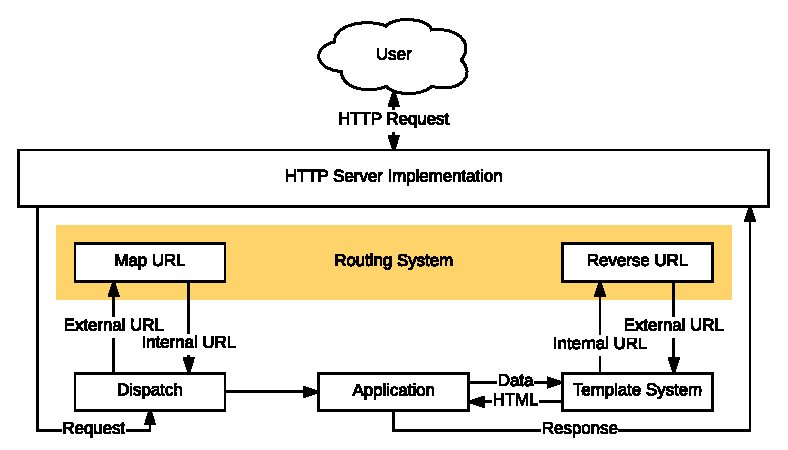
\includegraphics[width=\columnwidth]{request}
  \caption{Standard request life-cycle}
  \label{requestcycle}
\end{figure}

When a request is dispatched by Radiance, it first parses the request URL into an object presentation that makes it easier to modify. It then sends it through the routing system's mapping functions, which turn this external URL into an internal one. The request is then dispatched to the according application that ``owns'' the URL in the internal representation. \\

Since Radiance has full control over the organisation of the internal representation, it can make strict demands as to how applications need to structure their URLs. Specifically, it requires each application to put all of its pages on a domain that is named after their application. \\

In our sample application, we might write the view page something like this, where \texttt{blog/view} is the internal URL that the view page is reachable on.

\begin{minted}[fontsize=\small]{common-lisp}
(define-page view "blog/view" ()
  (render-template (template "view.html")
                   (get-post (get-var "post-id"))))
\end{minted}

If, as an administrator of an installation of this blog application, we now wanted to reach this page through the URL \texttt{www.example.com/blog/view}, the mapping route functions would have to strip away the \texttt{www.example.com} domain, recognise the \texttt{blog} folder, and put that as the URL's domain instead. We can achieve this relatively easily with the following definition.

\begin{minted}[fontsize=\small]{common-lisp}
(define-route blog :mapping (uri)
  (when (begins-with "blog/" (path uri))
    (setf (domains uri) '("blog")
          (path uri) (subseq (path uri) 5))))
\end{minted}

Alternatively, we could also use the even simpler string-based definition.

\begin{minted}[fontsize=\small]{common-lisp}
(define-string-route blog :mapping
  "/blog/(.*)" "blog/\\1")
\end{minted}

Naturally, if you wanted different behaviour depending on which domain the request came from, you'd have to write a more specific translation. \\

With the mapping alone the case is not yet solved, though. When a page is emitted that contains links, the links too must be translated, but in the opposite way. Unfortunately, because routes can be arbitrarily complex, it is not possible for the system to figure out a reversal route automatically. The logic of a reversal route will usually be much the same as it was for the mapping route and should thus not be a problem to figure out, though. \\

The reversal of URLs should receive special support from the templating system, as it is very frequently needed and should thus be short. Radiance does not dictate any specific template system, but offers extensions to some existing systems like Clip\cite{clip} to simplify this process. As a brief example, in Clip, URLs can be denoted through special attributes like this:

\begin{minted}[fontsize=\small]{html}
<a @href="blog/list">Latest Blog Posts</a>
<form method="post">
  <textarea name="text"></textarea>
  <input type="submit" @formaction="blog/submit" />
</form>
\end{minted}

The templating engine takes care of reading out the \texttt{@} attribute values, running them through the routing system's reversal functions, and putting the resulting URL into the corresponding attribute to produce a valid link.

\subsection{Environments}
Radiance's ``environment'' encapsulates the configuration of a Radiance installation. Through it, applications can provide settings that the administrator can set to their liking. It also provides the information necessary to figure out which implementation to use for an interface. \\

The environment itself simply dictates a directory that contains all of these configuration files. Each application in the system automatically receives its own directory in which it can store both configuration, and temporary data files. By simply switching out this environment directory, the system can then be loaded into completely different configurations, for example allowing you to easily keep ``development'' and ``production'' setups. \\

%% FIXME
Ideally, an administrator of a system will not have to touch any source code, and instead will be able to configure the system through a set of human-readable configuration files. It is, of course, still possible to configure the system through usual Lisp code, should one prefer this approach. \\

In our example application we might want to give the administrator the ability to define a global blog title. We could provide a default value for it like this:

\begin{minted}[fontsize=\small]{common-lisp}
(define-trigger startup ()
  (defaulted-config "Irradiant Blogs" :title))
\end{minted}

We need to stick this into a trigger, in order to defer the evaluation to when Radiance is being started up and the environment has been decided. During the loading of the system, the environment might not have been set yet, and we would not be able to access the configuration storage. \\

While Radiance does provide default implementations for all of its interfaces, it is likely that some of them are not usable for a production setting. In order to change, say, the database interface's implementation, we would then have to modify the Radiance core's configuration file. We can either modify the file directly like so:

\begin{minted}[fontsize=\small]{common-lisp}
((:interfaces (:database . "i-postmodern")
              ...)
 ...)
\end{minted}

.. or instead use the programmatical way, like so:

\begin{minted}[fontsize=\small]{common-lisp}
(setf (mconfig :radiance-core :interfaces :database)
      "i-postmodern")
\end{minted}

\texttt{i-postmodern} here is the name of a standard implementation of the database interface for PostgreSQL databases. \\

Routes can also be configured through the core configuration file. Our previous example mapping route could be set up in the configuration file like this.

\begin{minted}[fontsize=\small]{common-lisp}
((:routes (blog :mapping "/blog/(.*)" "blog/\\1"))
 ...)
\end{minted}

Radiance will take care of converting the configuration data into an actual route definition like we saw above. \\

Every application's individual configuration can be changed in much the same way.

\section{Conclusion}
Radiance provides a web framework that adjusts itself depending on how many features the application requires. By separating the applications from the implementations of these features with an interface, it allows the application programmer to write their software against a well-specified API, and retains the ability for the administrator to decide which implementation is most suitable for their setup. \\

By maintaining a strict separation of the URL namespace and providing an automated URL rewriting mechanism, Radiance allows for easy sharing of the namespace between an arbitrary number of applications, while at the same time giving the administrator a convenient way to modify the behaviour of the translation to fit their specific server configuration. \\

Through the environment system, Radiance standardises the way each application is configured by the administrator and how the system is pieced together when it is loaded. As a consequence of that it becomes trivial to switch between different setups of a Radiance installation. The simple, human-readable configuration format used allows even users without intimate knowledge of Lisp to set up an instance.

\section{Further Work}
Currently, while it is possible to dynamically load applications, it is not possible to dynamically unload them. Doing so is troublesome, as an application's system might potentially modify any other part of the Lisp process. However, if there is a constraint on what kind of changes can be rolled back, it should be possible to provide a usable form of this kind of feature. \\

Radiance also does not allow you to change the implementation of an interface on the fly. This has much the same problems as the previous issue. In addition, though, the system needs to ensure that all dependant applications, including optionally dependant ones, are reloaded to make macro redefinitions take effect. Furthermore, since some interfaces expose classes and instances thereof, the system would either have to be able to migrate objects between interface implementations, or somehow invalidate the old instances if they are retained in another part of the application. \\

Ultimately it should be made possible to switch out the environment of a Radiance installation on the fly, for example to switch between development and production setups without having to restart completely. Doing so could massively improve the time needed to discover differences between different setups.

\bibliography{paper}
\end{document}

%%% Local Variables:
%%% mode: latex
%%% TeX-command-extra-options: "-shell-escape"
%%% TeX-master: t
%%% TeX-engine: luatex
%%% End:
